\documentclass[letterpaper]{article}
\usepackage[utf8]{inputenc}
%\usepackage[ansinew]{inputenc}
\usepackage[spanish]{babel}
\usepackage{graphicx}

\begin{document}

\title{Anteproyecto3\\ Laboratorio de Microcontroladores ADCs y Puerto Serial}
\author{
 Marco Antonio Montero Chavarría Carné: A94000\\
  \and
  Francisco Molina Carné: B14194\\  
}
\maketitle

\section{Investigación Previa}
Para elaborar el graficador de señales se ocupa investigar algunas características del STM32F4, como la conversión analógico a digital(bloque ADC), el timer visto en el proyecto pasado y la clase de comunicaciones en modelo de control abstracto(bloque CDCACM). Adicionalmente se ocuparía el circuito mostrado en la figura \ref{circ1} como protección para el microcontrolador e investigar acerca de las librerías pyserial, matplotlib y csv.
\begin{figure}[hbtp]
\centering
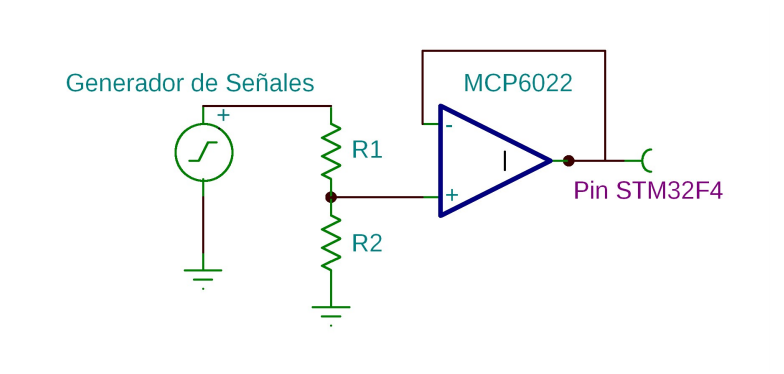
\includegraphics[width=12 cm]{circ1.png}
\caption{Circuito de protección}
\label{circ1}
\end{figure}

\newpage
\subsection{ADC}
En los microprocesadores de STM32x los ADC utilizan SAR(successive approximation register), un principio de conversión realizado por pasos. En este caso el número de steps son equivalentes al número de bits en el convertidor ADC, donde cada step se maneja por el reloj del ADC. Internamente el ADC maneja una estructura de capacitores  como la de la figura \ref{adc}. \cite{adcref}
\subsection{CDCACM}
La clase de comunicaciones para USB consiste en una clase que incluye una o más interfaces tales como interfaz de datos, audio o algunas relativas a almacenamiento masivo.\cite{wikicdc} En este caso se usa un modelo de control abstracto, un protocolo para emular puertos seriales por medio de USB y acceder al U-boot bootloader prompt.\cite{acmwiki} 

\subsection{PySerial}
PySerial es un módula que encapsula el acceso al puerto serial, proporciona el backend para python corriendo en Windows, Linux, BSD, Jython and IronPython (.NET y Mono). Para esto el módulo “serial” automáticamente selecciona el backend adecuado. Algunas características de la librería consisten en la misma interface para diferentes plataformas, soporta diferentes tamaños de bytes, bits de stop, paridad y control de flujo, es compatible con la librería io y trabaja con o sin timeout.\cite{pyserial} 


\subsection{Matplotlib}
Matplotlib es una librería de python para graficación en 2D que produce figuras con calidad de publicación en una variedad de formatos. Puede ser usada en scripts de python, python, el shell de ipython (ala MATLAB® or Mathematica®), aplicaciones para servidores web y otros toolkits de interface con el usuario. \cite{matplot} 


\subsection{Csv}
Librería para manejar los "Valores separados por coma", el formato más común para lectura y escritura de datos en hojas de cálculo, logs y bases de datos. Este módulo csv, implementa clases para leer y escribir en el formato de diferentes formas, como por ejemplo leer archivos con formate de Excel o bien escribir en el formato preferido por excel.\cite{csv} 

\newpage
\section{Solución Propuesta}
Se propone el esquema de la figura \ref{diag}.
\begin{figure}[hbtp]
\centering
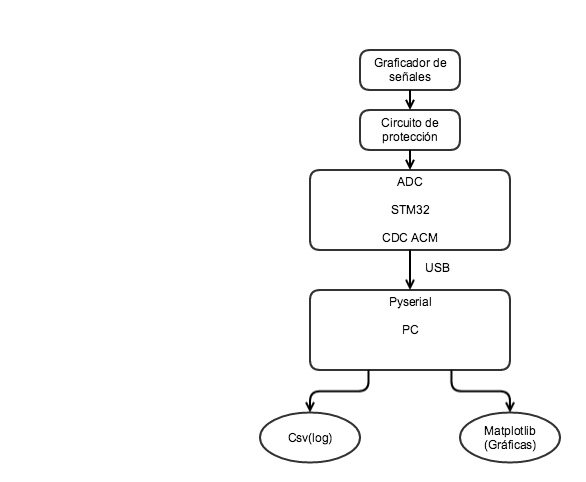
\includegraphics[width=10 cm]{flowdiag.png}
\caption{Diagrama de flujo del muestreo}
\label{diag}
\end{figure}


\section{Procedimiento}

En primera instancia hay que asegurarse que efectivamente la señal que envía el generador se encuentra en el rango de 5v y se procederá a elaborar el circuito de protección, verificando que la señal que entrará al pin del STM no sobrepase los 3V. Una vez comprobado que el circuito es seguro, entonces se conectará al microcontrolador para realizar el programa. \\[0.5cm] 
Utilizando la misma librería Open-Coroco \cite{coroco}, se utilizarán el bloque ADC para muestrear al doble o más de la frecuencia de la señal que envía el generador. Una vez tomados los datos, se ampliará el código para, por medio del CDCACM, enviar los datos por USB a la computadora. \\[0.5cm] 
Una vez que se compruebe que se envía los datos por medio de un programa de prueba, con un programa en Python se tomarán los datos del puerto por medio de la librería Pyserial y se graficará con Matplotlib al mismo tiempo que se guardan los datos en un log con la librería Csv.

\section{Observaciones y recomendaciones}

\begin{itemize}
\item Tener sumo cuidado con el circuito de protección, probar que las tensiones sean las adecuadas.
\item Realizar pequeñas pruebas antes de programar cada parte y descomponer el problema en problemas más sencillos.
\end{itemize}

\bibliographystyle{alpha} 
\bibliography{refs}



\end{document}
